\documentclass[a4paper]{report}

% Set page dimentions
\usepackage[margin=35mm]{geometry}

% Bibliography
\usepackage[numbers]{natbib}    % more bibliography options
\usepackage[nottoc]{tocbibind}  % add link to table of contents
\bibliographystyle{plainnat}    % more detailled plain bibliography

% Packages for french documents
\usepackage[french]{babel}  % latex rules for french words
\usepackage[utf8]{inputenc} % UTF-8 encoding for special chars
\usepackage[T1]{fontenc}    % T1 font for smooth render of special chars
\DeclareUnicodeCharacter{202F}{\thinspace}

% Define some colors
\usepackage{color}
\definecolor{string}{RGB}{100, 200, 0}
\definecolor{comment}{RGB}{150, 150, 150}
\definecolor{identifier}{RGB}{100, 100, 200}

% Source code style
\usepackage{listings}
\lstset{
	basicstyle=\footnotesize\ttfamily, % sets font style for the code
	frame=single,                 % adds a frame around the code
	showstringspaces=false,       % underline spaces within strings
	tabsize=4,                    % sets default tabsize to 2 spaces
	breaklines=true,              % sets automatic line breaking
	breakatwhitespace=true,       % sets if automatic breaks should only happen at whitespace
	keywordstyle=\color{magenta}, % sets color for keywords
	stringstyle=\color{string},   % sets color for strings
	commentstyle=\color{comment}, % sets color for comments
	emphstyle=\color{identifier}, % sets color for comments
}

% Appendices
\usepackage{appendix}
\renewcommand{\appendixname}{Annexe}
\renewcommand{\appendixtocname}{Annexes}

% Graphics
\usepackage{graphicx}        % images and figures
\usepackage{subcaption}      % subcaption and subtables
\graphicspath{ {assets} }    % path containing images
\usepackage{tikz}            % to generate graphics
\usetikzlibrary{arrows.meta} % setup arrows
\usetikzlibrary{chains,decorations.pathreplacing} % tiks chains
\tikzstyle{Arrow}=[-{Stealth[scale=1.5]}]

% Complex tables
\usepackage{multirow}
\usepackage{tabularx}
% Custom column types
\usepackage{array}
\newcolumntype{L}{>{\raggedright\arraybackslash}X} % Left-aligned auto-span columns
\newcolumntype{R}{>{\raggedleft\arraybackslash}X} % Right-aligned auto-span columns

% Localised number print (thousands, decimals, etc...)
\usepackage{numprint}

% Directory tree
\usepackage{dirtree}

% Acronyms
\usepackage[printonlyused,footnote]{acronym}

% Hyperlinks
\usepackage{xurl}                % allow word break for url wrapping
\usepackage[
  hidelinks,                     % invisible links
  pagebackref=true               % linkback to citations from bibliography
]{hyperref}                      % create clickable links
\usepackage{doi}                 % add links to doi urls

% Backrefs in the bibliography for french
\renewcommand{\backrefalt}[4]{
\ifcase #1 {}
  \or \emph{Cité page #2}
  \else \emph{Cité pages #2}
\fi
}
% Backref separators for french
\renewcommand{\backreftwosep}{ et~}
\renewcommand{\backreflastsep}{, et~}

% Style
\setlength{\parskip}{.3em} % space between paragraphs

% Custom commands
\newcommand{\btrfs}{BTRFS~\cite{rodeh2013btrfs}}
\newcommand{\erofs}{EROFS~\cite{gao2019erofs}}
\newcommand{\hptfs}{HPTFS~\cite{zhang2006hptfs}}
\newcommand{\ltfs}{LTFS~\cite{pease2010linear}}
\newcommand{\squashfs}{SquashFS~\cite{lougher2009squashfs}}
\newcommand{\udf}{UDF~\cite{optical2003universal}}

%--------------------------------------- Content ---------------------------------------%

\title{Système de fichiers pour le stockage d’informations numériques sur ADN}

\date{Octobre 2021}

\author{Nicolas Peugnet}

\begin{document}

\hypersetup{pageanchor=false}
\begin{titlepage}
\maketitle
\end{titlepage}

\hypersetup{pageanchor=true}
\tableofcontents

\chapter{Introduction}

Ce stage a été réalisé dans le cadre du projet DNA-Drive, un système développé par l'équipe de Stéphane Lemaire (\ac{lcqb}) visant à stocker des données numériques arbitraires via des molécules d'\ac{adn}.
Notre rôle sera de proposer un \emph{système de fichiers} adapté aux spécificités de ce nouveau médium de stockage.

\section{Systèmes de fichiers}

Le but principal d'un \emph{système de fichiers} est de permettre d'organiser des données sur un support de stockage.
En son absence, les différentes données d'un support seraient toutes écrites d'un seul tenant
et il ne serait pas possible de savoir où commence et où s'arrête un morceau cohérent de données.
Le système de fichiers offre donc la possibilité de répartir les données dans des segments nommés : les \emph{fichiers}.
Les fichiers peuvent être disposés au sein d'une arborescence de \emph{dossiers},
ce qui permet de les organiser de manière logique.
Les informations de cette arborescence sont des métadonnées que l'on doit donc stocker en plus des données.
Les systèmes de fichiers récents stockent en général bien plus de métadonnées que simplement les noms des fichiers et des dossiers.
Parmi celles-ci, on peut citer par exemple les dates de création et de modification,
ou bien encore les permissions lorsqu'il s'agit d'un système POSIX.

Grâce à cette structure d'arborescence de fichiers commune à tous les systèmes,
on obtient une compatibilité de l'un à l'autre,
ce qui offre à la couche supérieure une abstraction des supports de stockages.

Pour stocker ou lire des données, un système de fichiers doit communiquer avec le matériel.
Lorsqu'il s'agit d'un support de stockage classique respectant le \ac{lba},
comme c'est le cas des disque-durs et des \ac{ssd},
le système de fichiers n'a pas besoin de connaitre le fonctionnement détaillé du périphérique.
Il lui suffit de demander de lire ou écrire les données du bloc $n$
et c'est le contrôleur du périphérique lui-même qui se charge de retrouver l'emplacement physique de ce bloc logique.

Pour des supports plus spécifiques, il est assez fréquent que les systèmes de fichiers soient conçus exclusivement pour eux.
C'est par exemple le cas pour les bandes magnétiques avec \hptfs\ et \ltfs\ ou les disques optiques avec \udf.
Ces systèmes seront parfaitement adaptés à leur support et pourront donc pousser plus loin certaines optimisations.

\subsection{Fonctionnalités et caractéristiques}

En plus de son rôle d'abstraction des supports de stockage,
un système de fichier peut proposer un grand nombre de fonctionnalités et de caractéristiques intéressantes.
Nous n'introduirons ici que celles qui nous seront utiles pour la suite.

\paragraph{Type d'accès}
Un système de fichiers peut être accessible soit en lecture uniquement (\ac{ro}),
comme c'est le cas d'une bonne partie des systèmes compressés (\squashfs, \erofs, etc~\textellipsis),
soit en lecture et écriture (\ac{rw}) pour la grande majorité des autres systèmes.

\paragraph{Compression}
La compression peut avoir plusieurs intérêts pour un système de fichiers.
Elle peut bien-sûr permettre de réduire l'espace pris sur le support
et c'est ce cas d'usage que \squashfs\ tente d'optimiser.
Mais elle peut aussi servir à accélérer les opérations de lecture et d'écriture lorsqu'on est limité par la bande passante.
Les systèmes plus généralistes, comme \btrfs, utilisent la compression surtout dans ce but
et d'autres systèmes de fichiers, comme \erofs, sont même entièrement basés sur ce principe.

% TODO: quelles autres propriétés ?

\section{Stocker des données sur ADN}

L’\ac{adn} ou Acide DésoxyriboNucléique d’un organisme, constitue ce qu’on appelle le génome.
Le génome contient l’information génétique d’un organisme. L’\ac{adn} contient donc une information.
Cette information est codée sous la forme d’une suite de \emph{nucléotides}.
Un nucléotide est une molécule organique qui est l’élément de base de l’\ac{adn}.
Il existe quatre nucléotides différents qui sont représentés par quatre lettres : \textbf{A} pour Adénine, \textbf{C} pour Cytosine, \textbf{G} pour Guanine et \textbf{T} pour Thymine.
Nous pouvons voir directement le parallèle que nous pouvons faire entre l’\ac{adn} qui est une suite de nucléotides en base 4 et une donnée informatique qui est une suite de bits en base 2.

Il est donc naturel de penser à utiliser l’\ac{adn} pour stocker des données
et un certain nombre de démonstrations de faisabilité du stockage sur l’\ac{adn} ont été réalisées lors des dernières années.
Les travaux publiés pour l’instant se basent essentiellement sur l’utilisation d’\emph{oligonucléotides} qui sont des courts segments d’\ac{adn}.

\subsection{Encodages}

Les premières démonstrations significatives sur l’utilisation de ces oligonucléotides pour stocker des données remontent à seulement 2012 avec George Church \cite{church2012next} qui réussit à stocker 658~ko sur \numprint{54898} oligonucléotides.
Dans ses travaux, Church souhaite pouvoir contrôler le taux de GC et limiter les répétitions d’un même nucléotide.
Le taux de GC est la proportion de nucléotides G et C dans une séquence donnée. 
Les appariements GC ont trois liaisons hydrogène tandis que les appariements AT n'en ont que deux.
Un taux de GC élevé assure ainsi une meilleure stabilité, mais un taux trop élevé peut provoquer une autolyse (autodestruction) plus facilement.
Il est donc préférable d’avoir un taux de GC équilibré.
En ce qui concerne les longues répétitions d’un même nucléotide, elles produisent des erreurs lors du séquençage.
Pour toutes ces raisons, Church va utiliser un encodage en base 2 : $A=C=0$ et $T=G=1$ pour avoir plus de flexibilité (Table \ref{tab:church-encoding}).

\begin{table}[ht]
\centering
\setlength{\tabcolsep}{.8em}
\renewcommand\arraystretch{1.5}

\begin{subtable}[t]{.45\textwidth}
  \centering
  \begin{tabular}{|c|c|c|c|}
  \hline
  \multirow{2}{*}{\textbf{Bit}} & \textbf{0} & A & C \\
  \cline{2-4}
  & \textbf{1} & T & G \\
  \hline
  \end{tabular}
  \caption{Encodage Church}
  \label{tab:church-encoding}
\end{subtable}
\hfill
\begin{subtable}[t]{.54\textwidth}
  \centering
  \begin{tabular}{|c|c|c|c|}
  \cline{3-4}
  \multicolumn{2}{c|}{} & \multicolumn{2}{c|}{\textbf{Position}} \\
  \cline{3-4}
  \multicolumn{2}{c|}{} & \textbf{Paire} & \textbf{Impaire} \\
  \hline
  \multirow{2}{*}{\textbf{Bit}} & \textbf{0} & A & C \\
  \cline{2-4}
  & \textbf{1} & T & G \\
  \hline
  \end{tabular}
  \caption{Encodage BIODATA}
  \label{tab:biodata-encoding}
\end{subtable}

\caption{Différents encodages pour \ac{adn}}
\label{tab:dna-encodings}
\end{table}

Suite à ces travaux, un certain nombre de nouvelles publications vont apporter des améliorations intéressantes aux techniques existantes,
avec par exemple l'encodage de Goldman \cite{goldman2013towards} qui propose l'utilisation d'une base 3 (Figure \ref{fig:goldman-encoding}),
plus performante en densité de stockage.

\begin{figure}[ht]
\centering
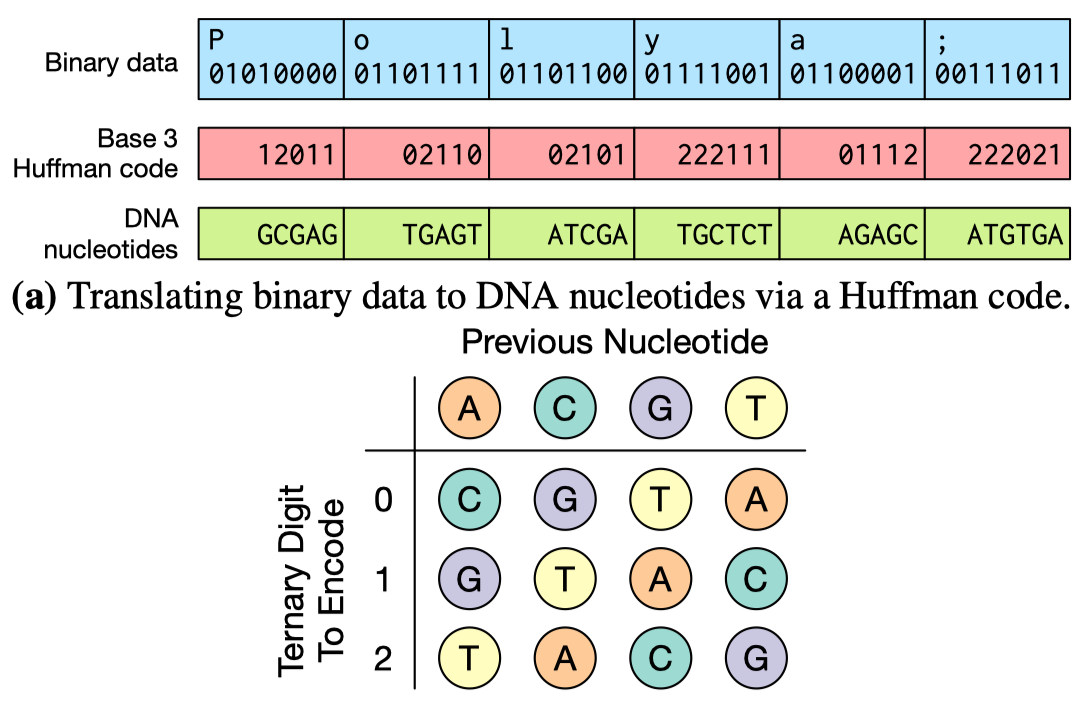
\includegraphics[width=.6\textwidth]{goldman-encoding}
\caption{Encodage de Goldman \cite{goldman2013towards}}
\label{fig:goldman-encoding}
\end{figure}


\subsection{Spécificités du DNA-Drive}

\subsubsection{Spécificités biologiques}

La spécificité principale de DNA-Drive par rapport à ses concurrents est d'utiliser la molécule d'\ac{adn} sous sa forme de double hélice, plutôt que sous la forme d'un simple brin.

Cette forme a plusieurs avantages.
Premièrement, la molécule est plus stable sous cette forme, ce qui limite sa dégradation et permet donc d'augmenter sa durée de vie.
Deuxièmement, il s'agit de la forme utilisée par l'ensemble des organismes vivants de notre planète\footnote{En considérant que les virus ne sont pas vivants},
ce qui nous permet donc potentiellement de profiter des mécanismes du vivant,
tels que la réparation automatique de l’\ac{adn} pour corriger les erreurs
ou la division cellulaire qui va permettre une copie peu coûteuse et très rapide de grandes quantités de données.

Cependant, faire en sorte qu'une molécule d'\ac{adn} soit compatible avec un être vivant lui ajoute des contraintes supplémentaires.
En particulier, en plus de garantir un taux de GC équilibré,
notre encodeur doit à tout prix éviter que les séquences de données, une fois encodées en ADN,
ne soient interprétés par l'hôte comme des séquences codantes de son génome.

Dans l'ADN d'un être vivant, ces parties codantes sont délimités par deux courtes séquences de nucléotides placées au début et à la fin de la zone à interpréter.
Il s'agit des codons START et STOP.
Le codon START indique le début d'une séquence à interpréter.
C'est donc celui qu'il faut à tout prix éviter d'obtenir une fois les données encodées.
Le codon STOP, au contraire, définit la fin d'une telle séquence.
Il est donc intéressant d'en insérer un maximum pour limiter la casse dans l'éventualité où un codon START aurait malencontreusement été ajouté.

En ce qui concerne la lecture des données, on utilise un séquenceur génétique portatif à
nanopore tels que celui utilisé par l’équipe de H. Yadzi \cite{yazdi2017portable} et présenté sur la Figure \ref{fig:oxford-nanopore-minion}.
Les séquenceurs en général ont un problème avec la lecture des homopolymères, c’est-à-dire des
séquences de répétitions d’un même nucléotide. On interdit donc les séquences de plus de trois fois
le même nucléotide pour éviter les erreurs de séquençage.

\begin{figure}[ht]
\centering
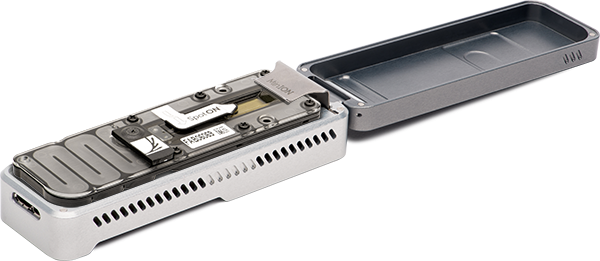
\includegraphics[width=.6\textwidth]{oxford-nanopore-minion}
\caption{Lecteur Oxford Nanopore MinION}
\label{fig:oxford-nanopore-minion}
\end{figure}

BIODATA, l'encodage mis au point par Clémence Blachon (\ac{lcqb}) pour le DNA-Drive est justement chargé de faire respecter ces propriétés par les données encodées.
Il est inspiré de celui de Church auquel des contraintes supplémentaires viennent s'appliquer :
Pour chaque bit, on fixe la valeur du nucléotide en fonction de sa valeur et de la parité de sa position (Table \ref{tab:biodata-encoding}).
De cette manière l'encodage est totalement contraint et le résultat est déterministe.
Les valeurs choisies garantissent quelle que soit la séquence de bits que :

\begin{itemize}
  \item Le taux de GC restera équilibré.
  \item Un nucléotide ne sera jamais répété plusieurs fois à la suite.
  \item Aucun codon START ne sera inséré.
  \item Des codons STOP seront insérés régulièrement.
\end{itemize}

Cet encodage nous permet donc de nous abstraire totalement des problématiques biologiques sous-jacentes lorsqu'on encode des données
et nous laisse ainsi la possibilité de stocker des valeurs complètement arbitraires.

\subsubsection{Spécificités techniques}

L'organisation physique des données du DNA-Drive est assez particulière et doit être prise en compte afin d'optimiser les lectures et les écritures.

\paragraph{Track} Une \emph{track} est un segment de données, actuellement de 1024~octets.
C'est la plus petite unité de stockage du système.
Toutes les écritures devront donc être alignées sur la taille d'une track.
Elles sont obtenues grâce à un assemblage MoClo \cite{werner2012fast} sur 3 niveaux
et sont refermées en un cercle pour former des \emph{plasmides}.
Cette forme particulière de la molécule d'\ac{adn} comporte plusieurs avantages.
Elle est tout d'abord plus pérenne grâce à sa structure circulaire,
car c'est principalement par ses extrémités que la molécule se dégrade.
Mais les plasmides profitent en plus de leur propre mécanisme d'auto-réplication autonome.
Cependant, cette forme ne permet pas de les mettre bout-à-bout,
il n'y a donc pas d'ordre naturel entre les tracks.
C'est pour cette raison que chaque track contient un \emph{barcode} qui permet de les identifier et donc de les réordonner.

\paragraph{Barcode} Le \emph{barcode} est un entier de 4~octets présent au tout début d'une track et permettant de l'identifier.

\paragraph{Pool} Un \emph{pool} est une minicapsule contenant plusieurs tracks.
Actuellement, un pool peut contenir \numprint{10000} tracks et les lectures sont réalisées par pool entier.
Il est possible de lire plusieurs pools en même temps
et même de fusionner des pools si les barcodes des tracks qu'ils contiennent ne se chevauchent pas.

\paragraph{Array} Un \emph{array} est une plaque de 96~pools ($8\times12$) qui est traditionnellement utilisée en biologie.
La taille maximum disponible pour des données d’un array est donc de \numprint{979.2}~Go ($96\times\numprint{10000}\times1020$~octets).
On peut multiplier les arrays afin d'obtenir une plus grande capacité de stockage.

Les chiffres donnés ici sur l’organisation du disque de 1024~octets par track et\numprint{10000}~tracks par pool sont limités respectivement par la complexité de l'assemblage MoClo et la précision limitée des techniques de séquençage actuelles
La capacité disponible est donc amenée à évoluer dans le futur avec l'arrivée de technologies plus performantes.

\section{Problématique}

Il existe donc plusieurs techniques et encodages permettant de stocker des informations arbitraires sur la molécule d'\ac{adn},
mais toutes ont en commun quelques inconvénients majeurs.
Ces inconvénients proviennent pour la plupart des limites actuelles des technologies de synthèse et de séquençage.
Une expérience d'un système automatisé de transmission de données par \ac{adn} datant de 2019 \cite{takahashi2019demonstration}
nous donne un ordre de grandeur des durées de lecture et d'écriture,
bien qu'il ne serait pas étonnant que des techniques plus performantes fassent leur apparition dans un futur proche :
La latence d'une opération d'écriture suivie d'une lecture d'une séquence de 12~octets est de 21~h,
dont \numprint{20.4}~h pour l'écriture (\numprint{8.4}~h de synthèse à 305~s par base et 12~h de stabilisation)
et les 36~min restantes pour la lecture (30~min de préparation et 6~min de séquençage et décodage).
Les lectures ne sont donc déjà pas très rapides, mais le point le plus limitant provient très largement des écritures qui sont exceptionnellement lentes, sans même parler de leur prix.

Une autre inconvénient du DNA-Drive et de l'ensemble des initiatives de stockage de données sur \ac{adn} est l'impossibilité de supprimer ou de modifier des données une fois écrites.
Ce point est particulièrement bloquant pour un système de fichiers \emph{ReadWrite} classique,
qui se base sur ces deux propriétés pour mettre à jour les fichiers et leurs métadonnées ainsi que pour récupérer de l'espace lorsque des fichiers sont supprimés.

Cette problématique se retrouve sur d'autres systèmes de stockages, comme les bandes magnétiques ou les disques optiques.
Elle est résolue par leur système de fichiers respectif, \ltfs\ pour les bandes magnétiques et \udf\ pour les CD et DVD non-RW.
Dans les deux cas le système est basé sur la réécriture complète des blocs modifiés des fichiers ainsi que de l'index dans le cas de \ltfs\ ou de la Virtual Allocation Table dans le cas de \udf.

% TODO: ajouter un § par rapport aux coût des écritures

La difficulté principale était donc de réussir à implémenter cette fonctionnalité sur un médium de stockage qui n'a pas la capacité de modifier les données existantes, tout en limitant les écritures au strict nécessaire.


\section{Réponse}

La proposition qui suit s'inscrit dans le cadre d'une réponse à court terme au problème posé.
Nous avons choisi de ne pas nous projeter trop loin dans le temps et avons donc basé l'ensemble de la réflexion sur les capacités actuelles des technologies de synthèse et de séquençage \ac{adn}.

L'objectif principal du système d'archivage de fichiers proposé est de réduire la quantité de données écrites, tout minimisant la quantité de données à lire pour récupérer les données.

Toutes les contraintes citées précédemment nous ont incité % TODO: j'aime bof ce mot
à nous orienter plus vers un système de sauvegardes que vers un véritable système de fichiers.
En effet, les vitesses et coûts d'écriture et de lecture ne permettent, pour le moment, absolument pas d'en faire un système de fichiers accessible à chaud.
Les cas d'usage envisagés seront donc ceux de sauvegardes sur différentes plages de temps : journalières, hebdomadaires ou mensuelles.
De cette manière, l'ensemble des opérations réalisés sur les fichiers pendant cette plage de temps seront factorisées dans un seul bloc de modification : la nouvelle version.
Ce n'est effectivement pas la peine d'écrire un fichier s'il va être supprimé ou renommé quelques secondes plus tard.

Afin de minimiser la quantité de données écrites par version, celles-ci sont réalisées de manière incrémentale.
Chaque nouvelle version est donc en quelque sorte une différence par rapport aux précédentes.
Ce stockage incrémental est obtenu grâce à une utilisation conjointe de la déduplication et de l'encodage delta.
De plus, comme aucune donnée ne peut être supprimée, nous en profitons pour réaliser un système versionné, qui nous laisse la possibilité d'accéder aux précédentes sauvegardes.




% TODO: write this §
La solution proposée se base sur une technique de  \cite{shilane2012wan}.

\chapter{Présentation générale}

% TODO: write this §
DNA-Backup tien donc plus 

Le système part du principe qu'on a une copie des données stockées en
\ac{adn} sur un support de stockage classique : le \emph{repo} (Figure \ref{fig:big-picture}).
\begin{figure*}[ht]
\centering

\begin{tikzpicture}

\draw (0,0) node[anchor=south west] {Ordinateur} rectangle (8, 3.5) ;

\draw (.5,1) rectangle (3,3) node[midway] {Source};
\draw (5,1) rectangle (7.5,3) node[midway] {Repo};
\draw (10,1) rectangle (12.5,3) node[midway] {DNA-Drive};

\draw[Arrow] (3,2) -- (5,2) node[midway,below] {Commit};
\draw[Arrow] (7.5,2) -- (10,2) node[midway,below] {Synthèse};

\end{tikzpicture}

\caption{Schéma global}
\label{fig:big-picture}
\end{figure*}

La Figure \ref{fig:repo-dir-tree} montre la structure du \emph{repo}. 

\begin{figure}
% \centering % centering ne fonctionne pas du tout avec le dirtree
\dirtree{%
.1 repo/.
.2 00000/.
.3 chunks/.
.4 000000000000000.
.4 000000000000001.
.4 000000000000002.
.4 000000000000003.
.3 files.
.3 hashes.
.3 recipe.
.2 00001/.
.3 chunks/.
.4 000000000000000.
.4 000000000000001.
.3 files.
.3 hashes.
.3 recipe.
}
\caption{Organisation du \emph{repo}}
\label{fig:repo-dir-tree}
\end{figure}

Pour un repo d'une taille totale de 401 Mio :

\begin{table}[ht]
\centering
\begin{tabular}{l r r}
\verb|repo/00000/recipe| &   5076011 &   1.2\% \\
\verb|repo/00000/files| &      24664 &   0.1\% \\
\verb|repo/00000/hashes| &   3923672 &   0.9\% \\
\verb|repo/00000/chunks| & 412263137 &  97.8\% \\
\verb|repo/00000| &        421287604 & 100.0\% \\
\end{tabular}
\caption{Répartition des données d'une première version}
\label{fig:repo-data-distribution}
\end{table}

\begin{itemize}
\item
  On considère que le \emph{repo} est toujours présent lors d'une
  écriture (\emph{commit}).
\item
  Le \emph{repo} peut être reconstruit à partir des données présentes
  dans le \emph{DNA-Drive}.
\item
  Les \emph{hashes} ne sont pas écrits en \ac{adn}, car ils peuvent être
  reconstruits à partir des données des \emph{chunks}.
\item
  L'ensemble des données écrites en \ac{adn} sont compressées, pour le moment
  via \emph{ZLib}.
\item
  Les métadonnées sont stockées de manière incrémentale, chaque version
  stocke donc ses métadonnées sous la forme de delta par rapport à la
  version précédente.
\end{itemize}

On imagine le \emph{DNA-Drive} comme un segment de \emph{pools} (Figure \ref{fig:data-layout})

\begin{figure}[ht]
\centering

\begin{tikzpicture}[
  start chain = going right,
  node distance = 0,
  Box/.style={draw, minimum width=2em, minimum height=2em, outer sep=0, on chain},
  Brace/.style={decorate,decoration={brace, amplitude=1em, raise=.5em, mirror}}
]
\node[Box] (p0) {$0$};
\node[Box] (p1) {$1$};
\node[Box] (p2) {$2$};
\node[Box] (p3) {$3$};
\node[Box] (p4) {$4$};
\node[Box,minimum width=6em] (ellipsis) {$\cdots$};
\node[Box] (p93) {$93$};
\node[Box] (p94) {$94$};
\node[Box] (p95) {$95$};

\draw[Arrow] (p4.east) to +(2em,0);
\draw[Arrow] (p93.west) to +(-2em,0);

\node (ver) at (0,-3.2em) {version};
\draw[->] (p0.south) to (ver);
\draw[Brace] (p1.south west) to node[black,midway,below=1.5em] {chunks} (p4.south east);
\draw[Brace] (p93.south west) to node[black,midway,below=1.5em,align=center] {metadata\\(recipe+files)} (p95.south east);

\end{tikzpicture}

\caption{Disposition des données}
\label{fig:data-layout}
\end{figure}


\chapter{Fonctionnement détaillé}

\section{Algorithme du commit}

\begin{enumerate}
\item
  Chargement des métadonnées du \emph{repo} afin de reconstruire en
  mémoire l'état de la dernière version :

  \begin{itemize}
  \item
    Reconstruction de la \emph{recipe} à partir des deltas de chaque
    version.
  \item
    Reconstruction du listage des fichiers à partir des deltas de chaque
    version (fichier \emph{files}).
  \item
    Reconstruction en mémoire des \emph{maps} de \emph{fingerprints} et
    de \emph{sketches} à partir des fichiers \emph{hashes} de chaque
    version.
  \end{itemize}
\item
  Listage des fichiers de la \emph{source}.
\item
  Concaténation de l'ensemble des fichiers de la source en un disque
  virtuel continu.
\item
  Lecture du \emph{stream} de ce disque virtuel et découpage en
  \emph{chunk} (de 8 Kio actuellement).
\item
  Pour chaque \emph{chunk} du \emph{stream} :

  \begin{enumerate}
  \item
    Calculer sa \emph{fingerprint} (hash classique), si elle est
    présente dans la \emph{map} : le stocker de manière dé-dupliquée
    (sous la forme d'identifiant faisant référence au \emph{chunk}
    trouvé dans la map).
  \item
    Sinon, calculer son \emph{sketch} (hash de ressemblance), s'il est
    présent dans la \emph{map}, le stocker sous la forme de delta
    (calcul de sa différence par rapport au \emph{chunk} trouvé dans la
    map).
  \item
    Sinon, le stocker sous la forme de nouveau bloc (ajout de sa
    \emph{fingerprint} et de son \emph{sketch} dans les \emph{maps} et
    stockage du contenu complet dans un nouveau \emph{chunk}).
  \end{enumerate}
\item
  Calcul des différences entre la nouvelle version et la précédente pour
  les métadonnées (\emph{files} et \emph{recipe}) et stockage des deltas
  ainsi obtenus.
\end{enumerate}

\section{Algorithme du restore}

\begin{enumerate}
\item
  Chargement des métadonnées du \emph{repo} afin de reconstruire en
  mémoire l'état de la dernière version :

  \begin{itemize}
  \item
    Reconstruction de la \emph{recipe} à partir des deltas de chaque
    version.
  \item
    Reconstruction du listage des fichiers à partir des deltas de chaque
    version.
  \end{itemize}
\item
  À partir de la \emph{recipe}, reconstruire le disque virtuel (sous la
  forme d'un \emph{stream}).
\item
  Découper ce \emph{stream} en fonction du listage des fichiers
  (\emph{files}) et réécrire les données dans les fichiers
  correspondants dans le répertoire \emph{destination}.
\end{enumerate}

\section{\texorpdfstring{Restaurer sans le
\emph{repo}}{Restaurer sans le repo}}

\subsection{\texorpdfstring{Reconstruction complète du
\emph{repo}}{Reconstruction complète du repo}}

Il est possible de reconstruire le \emph{repo} en entier en lisant la
totalité du \emph{DNA-Drive}.

\subsection{Restauration de la dernière
version}

Il est possible de ne restaurer que la dernière version en lisant dans
un premier temps le \emph{pool} de versions et les quelques \emph{pools}
de métadonnées (environ 2\% de la totalité des données écrites), puis en
lisant tous les \emph{pools} contenant des \emph{chunks} référencés par
la \emph{recipe} de cette version.

\subsection{Restauration d'un seul
fichier}

Il pourrait être possible (pas pour le moment) de ne restaurer qu'un
seul fichier d'une version en ayant moins de données à lire que pour
restaurer la version complète.

Pour cela, il faudrait en plus stocker en \ac{adn} un mapping \emph{chunk}
décompressé → \emph{pool} contenant ce \emph{chunk} et ainsi n'avoir à
lire que les \emph{pools} contenant des \emph{chunks} de ce fichier.

\chapter{Évaluation de performances}

Le dossier \verb|exp| contient les scripts permettant de reproduire
les expériences. Les scripts ne sont prévus pour fonctionner que sur
Linux.

On utilise le dépôt Git du noyau Linux comme base de donnée de test. Il
s'agit en effet d'une bonne simulation de modification de dossiers, car
l'historique contient toutes les modifications qui ont été apportées
petit à petit à l'ensemble des fichiers.

\section{Bases de comparaison}

Pour évaluer les performances du système DNA-Backup, quatre autres
systèmes de stockage versionnés ont été choisis comme base de
comparaison :

\begin{itemize}
\item
  \textbf{Git diffs}
\item
  \textbf{Git objects}
\item
  \textbf{Tar.gz}
\item
  \textbf{Taille réelle}
\end{itemize}

\subsection{Git diffs}

Ce système utilise le delta généré par la commande \verb|git diff|
pour sauvegarder une nouvelle version. Les données à stocker consistent
donc en une somme de deltas. Pour restaurer les données, il faut
appliquer séquentiellement l'ensemble des deltas jusqu'à obtenir l'état
de la version voulue.

\subsection{Git objects}

Ce système nous permet de simuler un système de fichiers qui ne serait
pas autorisé à modifier des données sur le support tout en gardant la
possibilité de modifier les données. Il s'agit de la manière dont Git
sauvegarde les données des fichiers d'un dépôt. Le contenu de chaque
fichier et de chaque dossier est hashé afin d'en obtenir une signature.
Il est ensuite compressé et stocké sous la forme d'\emph{object}
immuable, référencé par la signature obtenue. Si un fichier est modifié,
il produira une signature différente et sera donc stocké sous la forme
d'un nouvel \emph{object}. Par contre, si deux fichiers ont un contenu
strictement identique, ils produiront alors la même signature et seront
donc automatiquement dé-dupliqués. Les dossiers sont également stockés
en tant qu'\emph{objects}, mais les fichiers qu'ils contiennent sont
référencés non pas par leur nom, mais par leur signature. La
modification d'un fichier entrainera donc l'ajout de nouveaux
\emph{objects} pour l'ensemble des dossiers de la branche contenant ce
fichier. C'est de cette manière que Git est capable de créer un système
de fichiers modifiable à partir d'objets immuables.

\subsection{Tar.gz}

Une technique d'archivage assez classique à laquelle il peut être
intéressant de nous comparer est de stocker chaque version en tant
qu'une nouvelle archive Tar elle-même compressée à l'aide de Gzip. Cette
technique produit des archives d'une taille très réduite, car la
compression est appliquée à l'ensemble des fichiers d'un seul coup,
contrairement à une compression fichier par fichier.

Elle a cependant l'inconvénient de ne pas faire de dé-duplication ni
d'encodage delta, et ne tire donc pas du tout parti des données déjà
écrites sur le support.

\subsection{Taille réelle}

Cette base de comparaison n'est en réalité pas un système viable. Elle
correspond à la taille que prend en réalité le dossier \emph{source} au
moment de la sauvegarde. C'est un indicateur qui permet de se rendre
compte du poids que prendrait la sauvegarde de multiples versions sans
aucune déduplication ou compression.

\subsection{Tableau récapitulatif}

\begin{table*}[ht]

\begin{tabularx}{\textwidth}{L|L|L|L|L|L}

\textbf{Feature} &
\textbf{DNA-Backup} &
\textbf{Git diffs} &
\textbf{Git objects} &
\textbf{Tar.gz} &
\textbf{Taille réelle} \\
\hline

\multirow{2}{=}{Dé\-du\-pli\-ca\-tion} &
Niveau chunk &
\multirow{2}{=}{N/A} &
Niveau fichier &
\multirow{2}{=}{N/A} &
\multirow{2}{=}{N/A} \\ \cline{2-2} \cline{4-4}
& Transversal aux versions & & Transversal aux versions & \\
\hline

\multirow{2}{=}{Delta-encoding} &
Niveau chunk &
Niveau version &
\multirow{2}{=}{N/A} &
\multirow{2}{=}{N/A} &
\multirow{2}{=}{N/A} \\ \cline{2-3}
& Transversal aux versions & Par rapport à la précédente & & \\
\hline

Com\-pres\-sion &
Niveau chunk &
Niveau version &
Niveau fichier &
Niveau version &
N/A \\
\hline

Res\-tau\-ra\-tion de la dernière version &
Lecture des métadonnées puis des chunks de cette version (répartis dans différents pools) &
Lecture de la totalité du DNA-Drive &
Lecture récursive des différents objets composant la version (répartis dans différents pools) &
Lecture de la zone correspondant à la dernière version &
Lecture de la zone correspondant à la dernière version \\

\end{tabularx}

\caption{Tableau récapitulatif}
\label{tab:recap-table}
\end{table*}

\section{Nombre d'octets par version}

\subsection{Légende}

\begin{itemize}
\item
  \verb|4k_export| : le système DNA-Backup avec des blocs de 4 Kio.
\item
  \verb|8k_export| : le système DNA-Backup avec des blocs de 8 Kio.
\item
  \verb|diffs| : une somme de diffs Git minimales Gzippées.
\item
  \verb|nopack| : le dossier `objects de Git, contenant l'ensemble des
  données des fichiers et dossiers d'un dépôt.
\item
  \verb|targz| : une somme d'archives Tar Gzippées.
\item
  \verb|real| : le poids réel de chaque version et donc l'espace
  nécessaire à stocker l'ensemble des versions de manière
  non-dédupliquées.
\end{itemize}

\subsection{Résultats}


% TODO: use real data
\begin{table*}[ht]
\centering
\begin{tabularx}{\textwidth}{RRRRRRRR}
\textbf{Repo 4k} &
\textbf{Repo 8k} &
\textbf{DNA 4k} &
\textbf{DNA 8k} &
\textbf{Git diffs} &
\textbf{Git objects} &
\textbf{Tar.gz} &
\textbf{Taille réelle} \\
\hline
22 377 & 19 333 & 13 260 & 12 240 & 10 147 & 14 601 & 10 739 & 147 538 \\
2 374 & 3 138 & 3 060 & 4 080 & 1 768 & 2 573 & 11 304 & 149 715 \\
2 116 & 2 747 & 3 060 & 4 080 & 867 & 2 681 & 11 611 & 150 955 \\
3 012 & 2 917 & 4 080 & 4 080 & 869 & 2 359 & 12 111 & 152 087 \\
5 210 & 5 430 & 5 100 & 6 120 & 4 373 & 6 020 & 14 192 & 165 312 \\
\hline
35 089 & 33 565 & 28 560 & 30 600 & 18 024 & 28 234 & 59 957 & 765 607 \\

\end{tabularx}
\caption{Commits journaliers}
\label{tab:commits-daily}
\end{table*}


% TODO: use real data
\begin{table*}[ht]
\begin{tabularx}{\textwidth}{RRRRRRRR}
\textbf{Repo 4k} &
\textbf{Repo 8k} &
\textbf{DNA 4k} &
\textbf{DNA 8k} &
\textbf{Git diffs} &
\textbf{Git objects} &
\textbf{Tar.gz} &
\textbf{Taille réelle} \\
\hline
22 377 & 19 333 & 13 260 & 12 240 & 10 147 & 14 601 & 10 739 & 147 538 \\
2 374 & 3 138 & 3 060 & 4 080 & 1 768 & 2 573 & 11 304 & 149 715 \\
2 116 & 2 747 & 3 060 & 4 080 & 867 & 2 681 & 11 611 & 150 955 \\
3 012 & 2 917 & 4 080 & 4 080 & 869 & 2 359 & 12 111 & 152 087 \\
5 210 & 5 430 & 5 100 & 6 120 & 4 373 & 6 020 & 14 192 & 165 312 \\
\hline
35 089 & 33 565 & 28 560 & 30 600 & 18 024 & 28 234 & 59 957 & 765 607 \\

\end{tabularx}
\caption{Commits hebdomadaires}
\label{tab:commits-weekly}
\end{table*}


% TODO: use real data
\begin{table*}[ht]
\begin{tabularx}{\textwidth}{RRRRRRRR}
\textbf{Repo 4k} &
\textbf{Repo 8k} &
\textbf{DNA 4k} &
\textbf{DNA 8k} &
\textbf{Git diffs} &
\textbf{Git objects} &
\textbf{Tar.gz} &
\textbf{Taille réelle} \\
\hline
22 377 & 19 333 & 13 260 & 12 240 & 10 147 & 14 601 & 10 739 & 147 538 \\
2 374 & 3 138 & 3 060 & 4 080 & 1 768 & 2 573 & 11 304 & 149 715 \\
2 116 & 2 747 & 3 060 & 4 080 & 867 & 2 681 & 11 611 & 150 955 \\
3 012 & 2 917 & 4 080 & 4 080 & 869 & 2 359 & 12 111 & 152 087 \\
5 210 & 5 430 & 5 100 & 6 120 & 4 373 & 6 020 & 14 192 & 165 312 \\
\hline
35 089 & 33 565 & 28 560 & 30 600 & 18 024 & 28 234 & 59 957 & 765 607 \\

\end{tabularx}
\caption{Commits Mensuels}
\label{tab:commits-monthly}
\end{table*}


% Bibliography
\bibliography{doc.bib}

% Glossary
% LTeX: enabled=false

\chapter*{Glossaire}
\addcontentsline{toc}{chapter}{Glossaire}
\begin{acronym}
	\acro{cli}[CLI]{Command Line Interface}
	\acro{ltfs}[LTFS]{Linear Tape File System}
	\acro{udf}[UDF]{Universal Disk Format}
\end{acronym}


% Annexes
\appendix
\addappheadtotoc

\chapter{Documentation de la CLI}

DNA-Backup est un programme s'utilisant en \ac{cli}.
Trois commandes sont disponibles :

\begin{itemize}
  \item \verb|commit| : pour ajouter une nouvelle version au \emph{repo}.
  \item \verb|restore| : afin de restaurer la dernière version depuis le \emph{repo}
  \item \verb|export| : pour générer un export à partir des données du \emph{repo}
\end{itemize}


\end{document}
